\section{Fundamentos de estructuras metal óxido semiconductor}
La estructura MOS es la base de la tecnología moderna de 
circuitos integrados\cita{sze_physics_2007}
que componen las PCs, dispositivos móviles e infraestructura de comunicaciones.
Su forma de fabricación, denominada proceso CMOS,
ha permitido un crecimiento exponencial en la capacidad de cómputo,
gracias a la constante miniaturización de los transistores que componen un
circuito integrado (\figref{fig:moore}).
\fig{moore}{figuras/moore/moore.pdf}
{Reducción exponencial de las dimensiones del transistor.
La cantidad de transistores en un microprocesador se duplica cada dos años 
siguiendo la ley de Moore\cite{moore_cramming_2006}.
Reproducido de \cite{sedra_microelectronic_2010}.}
\subsection{Capacitor MOS}
Para entender el transistor MOS, estudiamos antes el capacitor MOS.
Su fabricación comienza con una oblea de alrededor de \SI{1}{\milli\meter} cortada de un monocristal de silicio.
Se oxida la superficie para obtener una delgada capa aislante de SiO$_2$.
Los detalles de este paso y los tratamientos posteriores
determinan una propiedad crucial de la interfaz Si-SiO$_2$:
la densidad de estados electrónicos superficiales.
Si su valor es muy alto, 
muchas propiedades eléctricas se ven degradadas 
(mayor ruido, corrimiento de parámetros con el tiempo).
El descubrimiento de cómo lograr una interfaz adecuada para transistores MOS
se dio décadas después de la idea original del transistor
\cite{chih-tang_evolution_1988}.

Sobre el óxido se deposita un conductor (\emph{gate}) 
como en la \figref{fig:cortemos}.
El mismo puede ser polisilicio (silicio policristalino) o,
en procesos recientes, un metal.
\fig{cortemos}{figuras/mos/corte.png}{Corte lateral de una estructura MOS. 
Reproducido de~\cite{sze_physics_2007}.}

Esta estructura forma un capacitor porque tiene dos conductores separados por un
dieléctrico.
%
\subsubsection{Estructura de bandas}
El análisis que sigue se basa en que las dimensiones laterales del MOS 
(paralelo a la superficie del sustrato) son mucho mayores que 
la longitud característica en que varían los campos en la dirección normal.
Esto permite considerarlo homogéneo en las direcciones laterales,
y limitarnos a un análisis unidimensional.

La \figref{fig:bandasmos} muestra la estructura de bandas del MOS ideal.
Un MOS ideal no tiene carga atrapada en el óxido ni en la interfaz
óxido-semiconductor, y sus bandas no tienen curvatura cuando no se le aplica
tensión.
Analizamos la variación de las bandas en la dirección normal al sustrato,
y su dependencia con la tensión $V$ aplicada.

Al conectar una fuente de tensión 
(por ejemplo una batería)
entre las terminales, 
fijamos la diferencia entre el nivel de Fermi del metal 
y el del semiconductor. 
El gradiente de $E_F$ produce un desplazamiento de cargas hasta que se llega a
una nueva condición de equilibrio (\figref{fig:polarizacionmos}).

%Bajo la condición $V=0$, los niveles de Fermi de metal y
%semiconductor coinciden.
%Para cada material, el nivel de vacío $\phi$ 
%está a una distancia fija del nivel de Fermi.
%En un metal esta distancia se denomina función trabajo.
%En un semiconductor esta cantidad es la suma de la afinidad electrónica $\xi$
%(distancia entre la banda de conducción y el nivel de vacío)
%y 
%Por ejemplo, la función trabajo del aluminio es \SI{4.2}{\volt} y la de una
%oblea dopada tipo P típica es \SI{3.6}{\volt}.
%Cuando coinciden los niveles de Fermi de metal y semiconductor, 
%difiere su potencial eléctrico en \SI{0.6}{\volt}.
%$\phi$ varía de forma contínua entre las terminales,
%curvando las bandas.
%Hace falta aplicar una tensión $V_{fb}=(\phi_m-\phi_s)/e$ 
%para obtener bandas planas (que implican, por Poisson, carga nula).
%
\fig{bandasmos}{figuras/mos/bandas.png}
{Estructura de bandas del capacitor MOS en flatband o bandas planas.
Reproducido de~\cite{sze_physics_2007}.}
\begin{figure}[H]
    \centering
    \begin{subfigure}[b]{.3\textwidth}
        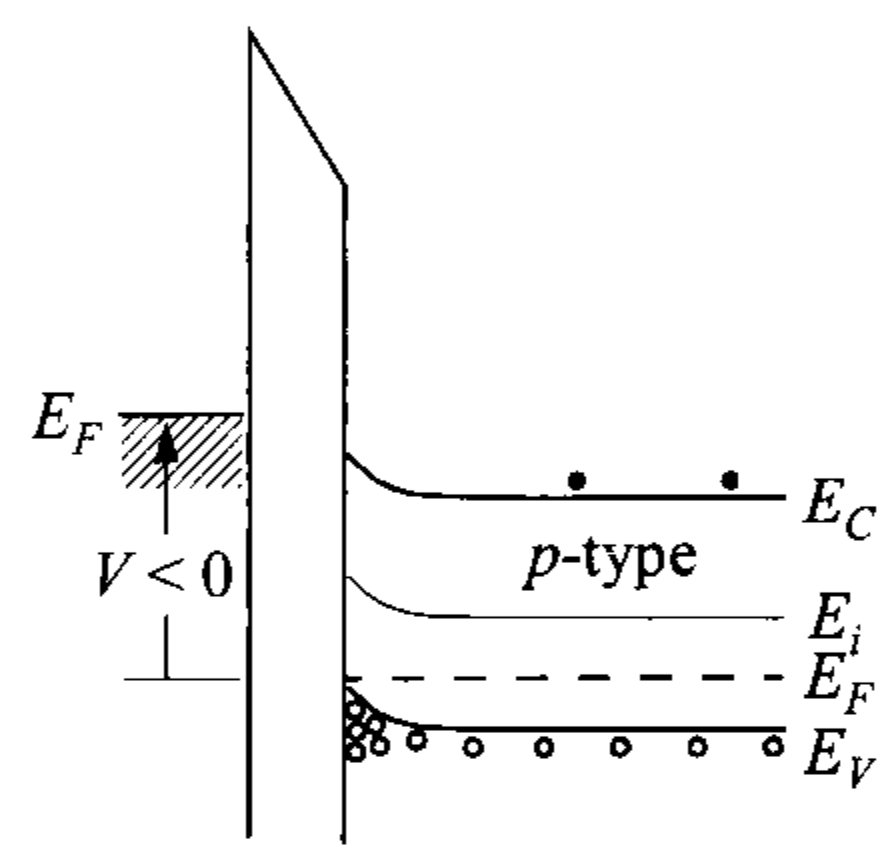
\includegraphics{figuras/mos/acumulacion.png}
        \label{fig:mosacumulacion}
        \caption{Acumulación}
    \end{subfigure}
    \begin{subfigure}[b]{.3\textwidth}
        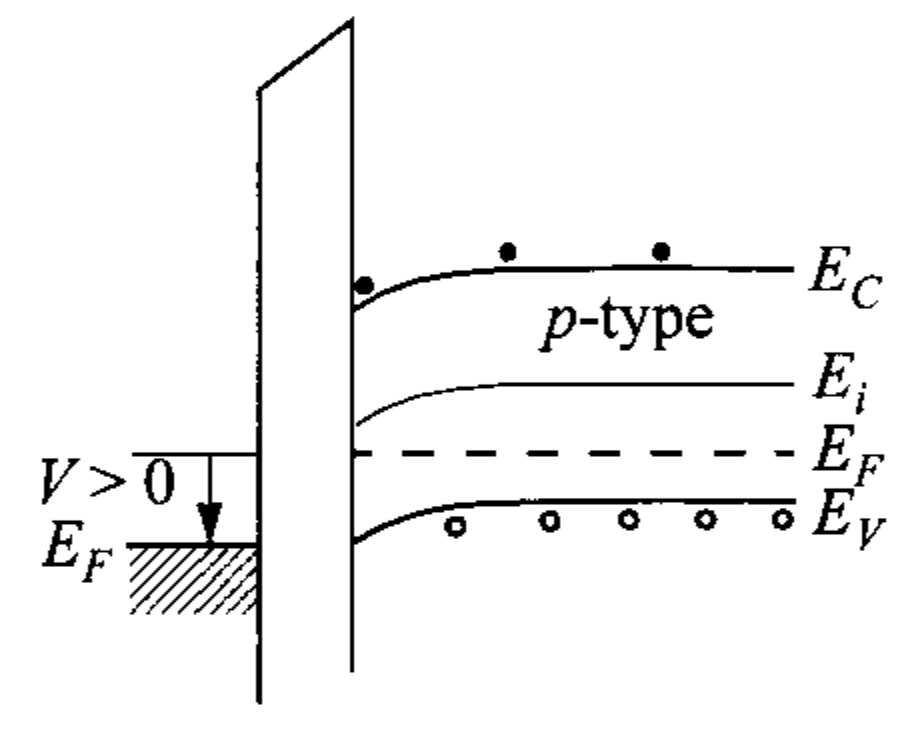
\includegraphics{figuras/mos/desercion.png}
        \label{fig:mosdesercion}
        \caption{Deserción}
    \end{subfigure}
    \begin{subfigure}[b]{.3\textwidth}
        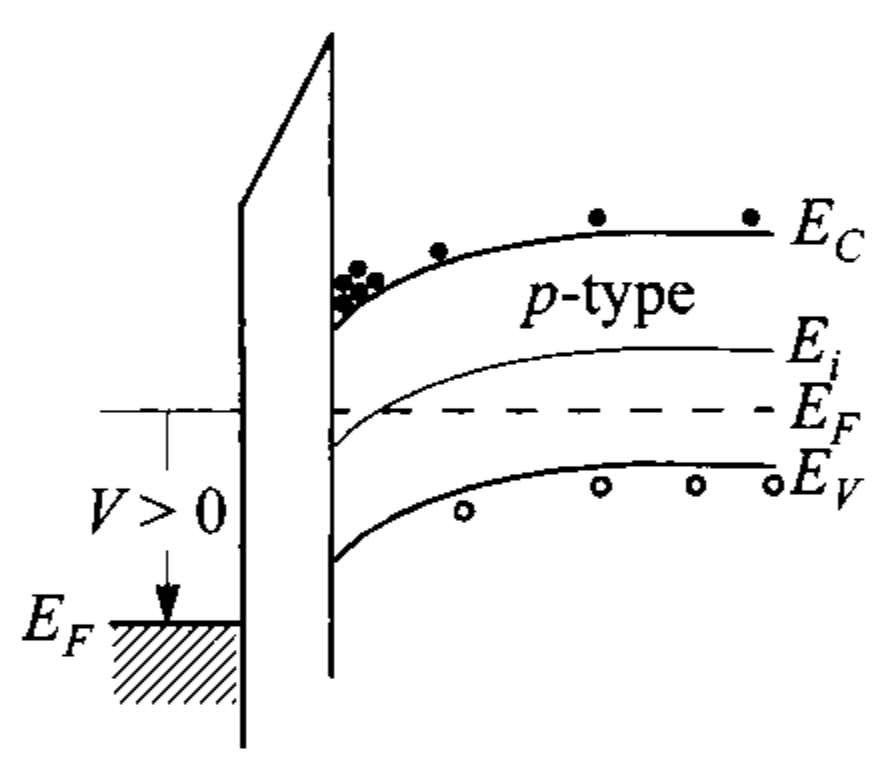
\includegraphics{figuras/mos/inversion.png}
        \caption{Inversión}
        \label{fig:mosinversion}
    \end{subfigure}
    \caption{Bandas del MOS polarizado, para $V_{fb}=0$.
Reproducido de~\cite{sze_physics_2007}.}
    \label{fig:polarizacionmos}
\end{figure}
%
\subsubsection{Concentración de portadores}
Para modelar la concentración de huecos y electrones en semiconductores,
se parte de la aproximación de electrón independiente.
La misma permite pensar en términos de niveles de 1 electrón que son ocupados
por electrones idénticos que no interactúan.
La termodinámica de un sistema así
lleva a la estadística de Fermi-Dirac, 
que dice que la probabilidad de ocupación de un nivel está dada por
\begin{align*}
    f(E) = \left[\exp\left(\frac{E-E_F}{kT}\right)+1\right]^{-1}
\end{align*}
con $E$ la energía del nivel y $E_F$ el nivel de Fermi.
$E_F$ es constante a lo largo de un sistema en equilibrio
químico,
y puede despejarse como función del número total de partículas.
Para eso se invierte la identidad $N=\sum_E f(E)$ donde la suma es sobre
todos los niveles de energía.

Para obtener la cantidad promedio de portadores en una banda,
es necesario sumar la ocupación de todos los niveles de la misma. 
En muchos casos de interés la banda de conducción cumple 
$|E-E_F| \gg kT$.
Esto permite aproximar
\begin{align*}
    f(E) = \exp\left(-\frac{E-E_F}{kT}\right)
\end{align*}.
Asimismo la suma de $f(E)$ sobre los niveles de la banda se puede aproximar
por una integral, y así se llega a las concentraciones de electrones y huecos
\begin{align*}
    n_c = N_c(T)e^{-\frac{\epsilon_c-E_F}{k_BT}}\\
    p_v = P_v(T)e^{-\frac{E_F-\epsilon_v}{k_BT}}
\end{align*} con $N_c(T)$ y $P_v(T)$ funciones que varían lentamente con la
temperatura.

Es conveniente expresar la concentración de portadores 
como función del potencial medido respecto del contacto de bulk
(un punto alejado del semiconductor, que tomamos como referencia):
$\psi_p=\phi(x)-\phi(\infty)$,
\begin{align}
    n &= n_0\exp\left(\frac{q\psi_p}{kT}\right)&
    p &= p_0\exp\left(-\frac{q\psi_p}{kT}\right),
    \label{eq:portadores_nodegenerados}
\end{align}
con $n_0$ y $p_0$ las concentraciones de portadores en el bulk.
\subsubsection{Impurezas}
Una parte central del proceso de fabricación
es introducir impurezas que aportan electrones o huecos
en regiones cuidadosamente controladas (\emph{doping}).
Así se crean zonas con concentraciones particulares de portadores.
La geometría y concentración de cada zona
es lo que define cada tipo de dispositivo 
que un proceso es capaz de producir.
Por ejemplo, un proceso puede estar diseñado para altas tensiones
eligiendo concentraciones y separaciones 
que logren una alta tensión de ruptura de las junturas.

Una técnica, llamada Chemical Vapor Deposition,
es exponer el sustrato a un gas
para que haya difusión de átomos del gas al sustrato.
La otra, llamada implantación, es ionizar las impurezas 
y acelerarlas mediante campos eléctricos hacia el sustrato.
Allí penetran hasta una profundidad que puede controlarse 
variando su energía\cite{campbell_science_2001}.


La forma en que las impurezas introducen portadores 
es capturando o emitiendo electrones.
Esto deja al átomo de impureza ionizado.
Para analizar este fenómeno se modela al efecto 
de una impureza con valencia 5
(uno más que el Silicio)
como si fuera un átomo normal de la red 
sumado a una carga fija +1, y un electrón.
Esta carga fija es capaz de atraer y formar estados ligados con electrones.
Usando la ecuación de masa efectiva\cite{datta_quantum_1989},
% FIXME: feo
se llega a que la energía de ligadura es muy baja
y por lo tanto las impurezas están casi totalmente ionizadas 
bajo condiciones normales de temperatura.
Esto se debe al efecto de la red: 
Por un lado actúa como dieléctrico
y apantalla el campo eléctrico de la carga.
Por otro lado altera la masa efectiva de los electrones 
y reduce la energía cinética y por lo tanto la potencial.

El análisis de impurezas aceptoras es análogo al de las donantes, 
con una carga fija -1 que se ioniza y libera un hueco.

Típicamente una región tiene al menos 
un órden de magnitud más impurezas de un tipo que del otro.
Se dice entonces que ahí los electrones o bien los huecos 
son el portador mayoritario.
En este caso la concentración de ese portador 
es aproximadamente igual a la concentración de su impureza.
La concentración del otro portador se encuentra fuertemente suprimida
debido al principio de Le Chatelier,
y vale aproximadamente $n_i^2/N_a$ 
con $n_i$ la concentración de portadores del semiconductor intrínsico (puro),
y $N_a$ la concentración de la impureza mayoritaria.

\subsubsection{Relación carga-tensión}
Planteando la ecuación de Poisson para el potencial $\phi$ en el semiconductor se llega a
\begin{align*}
    \deriv{^2\phi}{x^2} &= \frac e{\epsilon_s}(N_d-N_a+p-n),
\end{align*}
siendo los términos de la derecha concentraciones de donantes, aceptores,
huecos y electrones.


La aproximación~\ref{eq:portadores_nodegenerados} es válida para 
$|E_F-E_{c/v}|\gg kT$, 
o sea el nivel de Fermi alejado de los bordes de las bandas.
Así se obtiene un sistema de ecuaciones cuya solución para el campo eléctrico es
\begin{align*}
    \mathscr{E}_s &= \pm \frac{\sqrt 2kT}{qL_D}
    F(q\psi_p/kT,n_{p0}/p_{p0})\textnormal{, con}\\
    L_D^2&=\frac{kT\epsilon_s}{p_{p0}q^2}\textnormal{ , y}\\
    F(x,y) &= \sqrt{e^{-x}+x-1+y(e^x-x-1)}.
\end{align*}
Usando la ley de Gauss se obtiene la carga total del semiconductor
\begin{align*}
    Q_s = -\epsilon_s\mathscr{E}_s.
\end{align*}
La relación entre $V_G$ y $\psi_p$ viene de plantear la continuidad del vector
desplazamiento y la caída de tensión en el aislante
\begin{align*}
    V_G &= \psi_s + \mathscr{E}\frac{\epsilon_s}{\epsilon_{ox}}t_{ox}.
\end{align*}
Esto resulta en el gráfico de la \figref{fig:cargamos},
donde delimitamos distintos regímenes de operación.
%
\subsubsection{Regímenes de operación del capacitor MOS}
\begin{itemize}
    \item Acumulación:
        Aplicando tensión negativa al gate
        se puebla la superficie de portadores mayoritarios.
    \item Flatband/bandas planas: 
        A \SI{0}{\volt} la carga positiva de los huecos 
        (portadores mayoritarios)
        cancela la carga negativa de los aceptores, 
        entonces $Q=0$. 
    \item Deserción/Inversión débil:
        Aumentando la tensión se vacía la superficie de portadores
        mayoritarios,
        dejando la carga neta negativa de los aceptores ionizados.
    \item Inversión fuerte:
        Al cruzar $2\psi_B$ se puebla la superficie de portadores minoritarios
        con carga negativa,
        de igual magnitud y signo opuesto a la del sustrato.
        Un pequeño aumento adicional de $V_G$ resulta en un aumento exponencial
        de $|Q|$.
        Esta dependencia exponencial es válida hasta que el nivel de Fermi 
        se aproxima al borde de la banda de conducción y 
        el semiconductor se torna degenerado.
        Esto significa que se comporta como un metal,
        con una densidad de portadores que varía lentamente con el potencial.
\end{itemize}
\fig{cargamos}{figuras/mos/carga_vg.pdf}{Carga de un MOS típico 
    ($N_A=$\SI{4e15}{\centi\meter^{-3}}) en función
de la tensión de gate.
En la región de la izquierda el nivel de Fermi se acerca a la banda de
valencia. Esto torna degenerado al semiconductor y requiere el uso de
estadística de Fermi-Dirac en vez de aproximarla por Maxwell-Boltzmann.}
%
%
\subsection{Transistor MOS}
El transistor es la base de la electrónica moderna.
Modulando una señal con otra, 
permite realizar operaciones analógicas como amplificación y multiplicación.
Al operarlo con niveles discretos (prendido/apagado),
permite realizar las operaciones lógicas básicas (NOT, AND, etc.) que
se combinan para formar un circuito digital.
Su evolución permitió la integración de un número creciente de funciones
digitales y analógicas en un mismo circuito integrado.
%
\subsubsection{Modelo circuital}
El MOSFET o transistor MOS es un dispositivo con 4 terminales:
drain, gate, source y body (\figref{fig:mosfetschem}).
\fig{mosfetschem}{figuras/mos/mosfet.pdf}{Símbolo esquemático del transistor MOS.}
Frecuentemente se conecta source con body, rompiendo la simetría source-drain.
La tensión entre gate y source controla la corriente drain-source.

En la \figref{fig:mosfetoutput} se ven los 3 modos de operación del MOS:
\fig{mosfetoutput}{figuras/mos/output.pdf}{Curvas características de un
transistor MOS típico.}
\begin{itemize}
    \item Corte: Si $V_g<V_T$, no fluye corriente de drain.
        Por eso esta es denominada la ``tensión umbral''.
        $V_T$ es un parámetro de fabricación que ronda \SI{.3}{\volt} en procesos CMOS
        modernos.
        Un modelo más preciso es que $I_d$ depende exponencialmente de $V_g$.
    \item Triodo: Si $V_g>V_T$ y $V_{ds}<V_g-V_T$, la corriente de drain crece con la
        tensión drain-source siguiendo
        \begin{align*}
            I_D&=\beta_n\frac WL(V_{gs}-V_T-\frac{V_{ds}}2)V_{ds},
        \end{align*}
        con $\beta_n$ un parámetro del proceso y $\frac WL$ la relación de
        aspecto del MOSFET.
    \item Saturación: Si $V_g>V_T$ y $V_{ds}>V_g-V_T$ la corriente se mantiene, a primer
        orden, al valor constante
        \begin{align*}
            I_{Dsat}&=\frac{\beta_n}2\frac WL(V_{gs}-V_T)^2.
        \end{align*}
\end{itemize}
%
\subsubsection{Modelado físico}
El MOSFET de canal n consiste en un capacitor MOS de sustrato p entre dos regiones fuertemente dopadas 
tipo n, 
que forman drain y source (\figref{fig:mosfetestructura}).
Sin tensión de gate no puede fluir corriente entre drain y source porque una de las
junturas p-n (drain-sustrato o source-sustrato) queda polarizada en inversa.

Al polarizar el MOS en inversión se forma junto al óxido de gate 
una capa de electrones libres llamada canal.
Esta región de tipo n conecta drain y source y permite el flujo de corriente.
Al variar la tensión de gate, la variación de carga en el canal modula su
conductividad.
\fig{mosfetestructura}{figuras/mos/mosfet.png}{Estructura del transistor MOS.
Reproducido de~\cite{sze_physics_2007}.}
